
\begin{name}
	{Biên soạn: Thầy Phạm Tuấn, Nguyễn Cường \& Phan Văn Thành}
	{KSCL Lớp 12, PTTH Đội Cấn Vĩnh Phúc, 2020-2021}
\end{name}
\setcounter{ex}{0}
\Opensolutionfile{ans}[ans/ans-2-GHK1-21-KSCLDoiCanVinhPhuc-21]
\begin{ex}%[KSCL  PTTH Đội Cấn Vĩnh Phúc, 2020-2021]%[Phạm Tuấn, EX3-2021]%[2D1Y1-2]
Cho hàm số $f(x)$ có bảng biến thiên 
\begin{center}
	\begin{tikzpicture}
		\tkzTabInit[espcl=2.5,lgt=1.5,nocadre=false]
		{$x$/0.7,$y'$/0.7,$y$/2.1}
		{$-\infty$,$-2$, $3$,$+\infty$}
		\tkzTabLine{,+,0,-,0,+}
		\tkzTabVar{-/$-\infty$,+/$1$,-/$0$,+/$+\infty$}
		\begin{scope}[on background layer]\path[white]node{MDD-108};\end{scope}
\end{tikzpicture}
\end{center}
Hàm số đã cho đồng biến trên khoảng nào dưới đây?
\choice
{$(-\infty;1)$}
{\True  $(3;5)$}
{$(-2;3)$}
{$(0;+\infty)$}
\loigiai{
Từ bảng biến thiên suy ra hàm số đồng biến trên khoảng $(3;5)$.
}
\end{ex}

\begin{ex}%[KSCL  PTTH Đội Cấn Vĩnh Phúc, 2020-2021]%[Phạm Tuấn, EX3-2021]%[1D2Y2-1]
Có bao nhiêu cách sắp xếp $5$ học sinh thành một hàng dọc?
\choice
{$5^5$}
{\True $5!$}
{$4!$}
{$5$}
\loigiai{
Mỗi cách sắp xếp là một hoán vị của $5$ học sinh. Do đó có $5!$ cách.
}
\end{ex}

\begin{ex}%[KSCL  PTTH Đội Cấn Vĩnh Phúc, 2020-2021]%[Phạm Tuấn, EX3-2021]%[2D1Y5-1]
\immini{
Hàm số nào dưới đây có đồ thị như đường cong ở hình vẽ
\choice
{$y=x^3-3x+1$}
{\True $y=-x^3+3x+1$}
{$y=x^3+x+1$}
{$y=x^3-3x+1$}
}
{
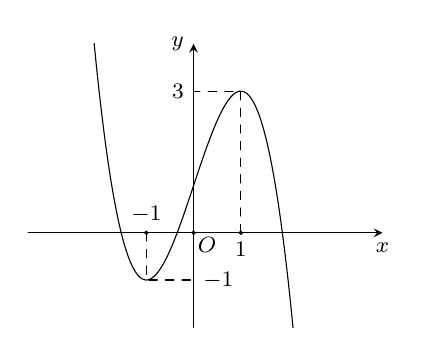
\begin{tikzpicture}[scale=0.6, font=\footnotesize, line join=round, line cap=round, >=stealth]
\draw[->] (-3.5,0)--(4,0) node[below]{$x$} ;
\draw[->] (0,-2)--(0,4) node[left]{$y$};
\draw[fill=black] (0,0) circle(1pt) node[below right=-2pt] {$O$} ;
\draw (1,0) circle(1pt) node[below]{$1$} (-1,0) circle(1pt) node[above]{$-1$} (0,-1) node[right]{$-1$} (0,3) node[left]{$3$};
\draw[dashed] (-1,0)--(-1,-1)--(0,-1) (1,0)--(1,3)--(0,3);
\clip (-3.5,-2) rectangle (4,4) ;
\draw[smooth, samples=100, domain=-3.5:5] plot(\x,{-1*(\x)*(\x)*(\x) + 3*(\x)+1}) ;
\end{tikzpicture}
}
\loigiai{
Ta thấy đồ thị hàm số đi qua các điểm $(-1;-1)$ và $(1;3)$. \\
Do đó hàm số đã cho là $y=-x^3+3x+1$.
}
\end{ex}

\begin{ex}%[KSCL  PTTH Đội Cấn Vĩnh Phúc, 2020-2021]%[Phạm Tuấn, EX3-2021]%[2D1Y5-1]
\immini{Đường cong ở hình bên là đồ thị của một trong bốn hàm số đưới đây. Hàm số đó là hàm số nào?
\choice
{$y=x^3-x^2-1$}
{$y=-x^4+x^2-1$}
{$y=-x^3+x^2-1$}
{\True $y=x^4-x^2-1$}
}
{
\begin{tikzpicture}[scale=0.8, font=\footnotesize, line join=round, line cap=round, >=stealth]
\draw[->] (-3,0)--(3,0) node[below]{$x$} ;
\draw[->] (0,-1.5)--(0,1.5) node[left]{$y$};
\draw[fill=black] (0,0) circle(1pt) node[above left=-2pt] {$O$} ;
%\draw (1,0) circle(1pt) node[above]{$1$} (-1,0) circle(1pt) node[above]{$-1$} (0,-4) node[above left]{$-4$} (0,-3) node[above left]{$-3$};
\clip (-3,-4.5) rectangle (3,1.5) ;
\draw[smooth, samples=100, domain=-3:3] plot(\x,{(\x)*(\x)*(\x)*(\x) - (\x)*(\x)-1}) ;
\end{tikzpicture}
}
\loigiai{
Từ đồ thị suy ra hàm số là $y=x^4-x^2-1$.
}
\end{ex}

\begin{ex}%[KSCL  PTTH Đội Cấn Vĩnh Phúc, 2020-2021]%[Phạm Tuấn, EX3-2021]%[2H1Y2-3]
Hình chóp tứ giác đều có bao nhiêu mặt phẳng đối xứng?
\choice
{\True $4$}
{$3$}
{$6$}
{$2$}
\loigiai{
Hình chóp tứ giác đều có $4$  mặt phẳng đối xứng.
}
\end{ex}

\begin{ex}%[KSCL  PTTH Đội Cấn Vĩnh Phúc, 2020-2021]%[Phạm Tuấn, EX3-2021]%[2D1Y2-2]
\immini{
Cho hàm số $y=f(x)$ có đồ thị như hình bên.
Giá trị cực đại của hàm số bằng?
\choice
{$1$}
{\True $3$}
{$2$}
{$-1$}
}
{
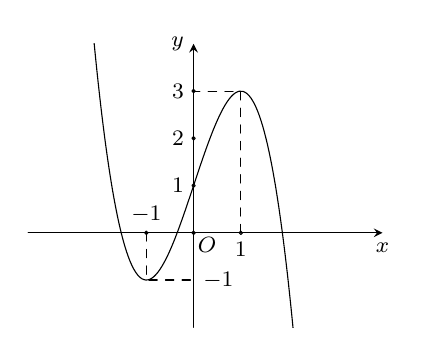
\begin{tikzpicture}[scale=0.6, font=\footnotesize, line join=round, line cap=round, >=stealth]
\draw[->] (-3.5,0)--(4,0) node[below]{$x$} ;
\draw[->] (0,-2)--(0,4) node[left]{$y$};
\draw[fill=black] (0,0) circle(1pt) node[below right=-2pt] {$O$} ;
\draw (1,0) circle(1pt) node[below]{$1$} (-1,0) circle(1pt) node[above]{$-1$} (0,-1) node[right]{$-1$} (0,3) circle(1pt) node[left]{$3$} 
(0,2) circle(1pt)node[left]{$2$} (0,1) circle(1pt)node[left]{$1$} ;
\draw[dashed] (-1,0)--(-1,-1)--(0,-1) (1,0)--(1,3)--(0,3);
\clip (-3.5,-2) rectangle (4,4) ;
\draw[smooth, samples=100, domain=-3.5:5] plot(\x,{-1*(\x)*(\x)*(\x) + 3*(\x)+1}) ;
\end{tikzpicture}
}
\loigiai{
Từ đồ thị hàm số suy ra giá trị cực đại bằng $3$.
}
\end{ex}

\begin{ex}%[KSCL THPT Đội Cấn - Vĩnh Phúc, 2021]%[Nguyễn Cường, 12EX3]%[1D5Y2-1]
Cho hàm số $y=\dfrac{x+2}{x-1}$. Tính $y'(3)$.
	\choice
	{$\dfrac{5}{2}$}
	{$\dfrac{3}{4}$}
	{$-\dfrac{3}{2}$}
	{\True $-\dfrac{3}{4}$}
	\loigiai{
Tập xác định $\mathscr{D}=\mathbb{R}\setminus \{1\}$.\\
Đạo hàm $y'=\dfrac{-3}{(x-1)^2}\Rightarrow y'(3)=-\dfrac{3}{4}$.
}
\end{ex}

\begin{ex}%[KSCL THPT Đội Cấn - Vĩnh Phúc, 2021]%[Nguyễn Cường, 12EX3]%[2H1Y3-2]
Cho khối tứ diện $OABC$ có $OA$, $OB$, $OC$ đôi một vuông góc và $OA=3$ cm, $OB=4$ cm, $OC=10$ cm. Thể tích khối tứ diện $OABC$ bằng
	\choice
	{\True $20$ cm$^3$}
	{$10$ cm$^3$}
	{$40$ cm$^3$}
	{$120$ cm$^3$}
	\loigiai{
\immini{
Thể tích khối tứ diện $OABC$ là $V=\dfrac{1}{3}\cdot OA\cdot \dfrac{1}{2}\cdot OB\cdot OC=20$ cm$^3$.
}
{
\begin{tikzpicture}[=>stealth,line join=round,line cap=round, font=\footnotesize, scale=.7]
\def\a{4}
\def\goc{210}
\def\b{2.5}
\def\h{4}
\path
(0,0)coordinate (O)++(0:\a)coordinate (B)++(\goc:\b)coordinate (C)
(O)++(90:\h)coordinate (A)
;
\draw (A)--(O)--(C)--(B)--cycle
(A)--(C)
;
\draw[dashed] (O)--(B);
\foreach \x/\g in{A/90,B/45,C/-60,O/180}
\fill[black](\x)circle(1.5pt) ($(\x)+(\g:3mm)$)node{$\x$}
;
\end{tikzpicture}
} 
}
\end{ex}

\begin{ex}%[Khảo sát Toán 12 - THPT Đội Cấn -Vĩnh Phúc - 21]%[Phan Văn Thành]%[2H1Y2-2]
	Có bao nhiêu loại khối đa diện đều?
	\choice
	{\True $ 5 $}
	{$  2 $}
	{$ 4  $}
	{$ 3 $}
	\loigiai{
		Có $5$ khối đa diện đều gồm 
		\begin{itemize}
			\item Loại $\{3,3\}$ là khối tứ diện đều.
			\item Loại $\{4,3\}$ là khối lập phương.
			\item Loại $\{3,4\}$ là khối bát diện đều.
			\item Loại $\{5,3\}$ là khối mười hai mặt đều.
			\item Loại $\{3,5\}$ là khối hai mươi mặt đều.
		\end{itemize}
		
	}
\end{ex}

\begin{ex}%[KSCL  PTTH Đội Cấn Vĩnh Phúc, 2020-2021]%[Phạm Tuấn, EX3-2021]%[2D1B1-1]
Trong các hàm số sau hàm số nào nghịch biến trên tập số thực?
\choice
{$y=x^{2}-5 x+6$}
{\True $y=-x^{3}+2 x^{2}-10 x+4$}
{$y=x+5$}
{$y=\dfrac{x+10}{x-1}$}
\loigiai{
Xét hàm số $y=-x^{3}+2 x^{2}-10 x+4$.  \\
Ta có $y' = -3x^2 +4x -10 <0$, $\forall x \in \mathbb{R}$. \\
Do đó hàm số nghịch biến trên tập số thực.
}
\end{ex}

\begin{ex}%[KSCL  PTTH Đội Cấn Vĩnh Phúc, 2020-2021]%[Phạm Tuấn, EX3-2021]%[2D1B5-3]
\immini{Cho hàm số $y=f(x)$ có đồ thị như hình vẽ bên.
Phương trình $2f(x)+7 =0$ có bao nhiêu nghiệm?
\choice
{Vô nghiệm}
{\True $4$}
{$3$}
{$2$}
}
{
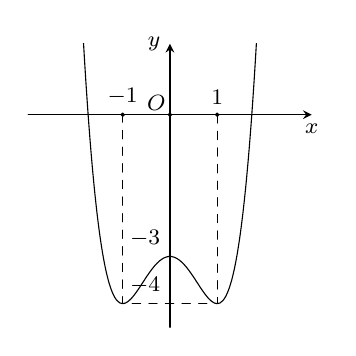
\begin{tikzpicture}[scale=0.6, font=\footnotesize, line join=round, line cap=round, >=stealth]
\draw[->] (-3,0)--(3,0) node[below]{$x$} ;
\draw[->] (0,-4.5)--(0,1.5) node[left]{$y$};
\draw[fill=black] (0,0) circle(1pt) node[above left=-2pt] {$O$} ;
\draw (1,0) circle(1pt) node[above]{$1$} (-1,0) circle(1pt) node[above]{$-1$} (0,-4) node[above left]{$-4$} (0,-3) node[above left]{$-3$};
\draw[dashed] (1,0)--(1,-4)--(-1,-4)--(-1,0);
\clip (-3,-4.5) rectangle (3,1.5) ;
\draw[smooth, samples=100, domain=-3:3] plot(\x,{(\x)*(\x)*(\x)*(\x) - 2*(\x)*(\x)-3}) ;
\end{tikzpicture}
}
\loigiai{
Ta có $2f(x)+7=0 \Leftrightarrow f(x) = - \dfrac{7}{2}$. \\
Số nghiệm của phương trình là số giao điểm của đồ thị hàm số $y=f(x)$ và đường thẳng $y=- \dfrac{7}{2}$. \\
Do đó phương trình đã cho có $4$ nghiệm phân biệt.
}
\end{ex}

\begin{ex}%[KSCL  PTTH Đội Cấn Vĩnh Phúc, 2020-2021]%[Phạm Tuấn, EX3-2021]%[1D3B3-3]
Cho một cấp số cộng $(u_n)$  với $u_1 = 5$ và $u_3=1$. Khi đó số hạng $u_2$ của cấp số cộng đã cho là
\choice
{$2$}
{\True $3$}
{$-2$}
{$6$}
\loigiai{
Gọi $d$ là công sai. Ta có $u_3-u_1 = 2d \Rightarrow d = -2$. \\
Suy ra $u_2 = u_1+d =3$.
}
\end{ex}

\begin{ex}%[KSCL  PTTH Đội Cấn Vĩnh Phúc, 2020-2021]%[Phạm Tuấn, EX3-2021]%[2H1B3-2]
Cho khối chóp tam giác đều có cạnh đáy bằng $2$ và chiều cao $h =12$. Thể tích của khối chóp đã cho bằng
\choice
{$6\sqrt{3}$}
{\True  $4\sqrt{3}$}
{$12\sqrt{3}$}
{$24\sqrt{3}$}
\loigiai{
Thể tích của khối chóp đã cho bằng $V= \dfrac{1}{3} \cdot 12  \cdot \dfrac{\sqrt{3}}{4} \cdot 2^2 = 4\sqrt{3}$.
}
\end{ex}

\begin{ex}%[KSCL  PTTH Đội Cấn Vĩnh Phúc, 2020-2021]%[Phạm Tuấn, EX3-2021]%[1D5B2-3]
Viết phương trình tiếp tuyến của đồ thị hàm số $y= x^2-x+5$ biết tiếp tuyến đó vuông góc với đường
thẳng $y=-\dfrac{1}{3}x +1$.
\choice
{$y=3x-13$}
{$y=3x+13$}
{\True $y=3x+1$}
{$y=3x-1$}
\loigiai{
Gọi $x_0$ là hoành độ của tiếp điểm.  \\
Ta có $y'(x_0) = 2x_0-1$. Tiếp tuyến vuông góc với đường thẳng $y=-\dfrac{1}{3}x +1$, suy ra
\[
y'(x_0) \cdot \left (-\dfrac{1}{3} \right ) =-1 \Leftrightarrow 2x_0-1  =3 \Leftrightarrow x_0 =2.
\]
Phương trình tiếp tuyến là $y= 3(x-2)+ 7 = 3x +1$.
}
\end{ex}

\begin{ex}%[KSCL  PTTH Đội Cấn Vĩnh Phúc, 2020-2021]%[Phạm Tuấn, EX3-2021]%[2D1B4-1]
Đồ thị hàm số $y=\dfrac{\sqrt{1-x^2}}{x^2+2x}$ có số đường tiệm cận bằng
\choice
{\True $1$}
{$2$}
{$3$}
{$4$}
\loigiai{
Tập xác định $\mathscr{D} = [-1;1] \setminus  \{0\}$. Suy ra đồ thị hàm số đã cho không có tiệm cận ngang. \\
Ta có  $\displaystyle \lim_{x\to 0^+} \dfrac{\sqrt{1-x^2}}{x^2+2x} = +\infty$.  \\
Do đó đồ thị hàm số đã cho chỉ có duy nhất một đường tiệm cận $x=0$.
}
\end{ex}

\begin{ex}%[KSCL  PTTH Đội Cấn Vĩnh Phúc, 2020-2021]%[Phạm Tuấn, EX3-2021]% [2H1B3-2]
 Cho khối lăng trụ tam giác đều có tất cả các cạnh bằng $a$. Thể tích khối lăng trụ tam giác đều đã
cho bằng
\choice
{\True $\dfrac{a^3\sqrt{3}}{4}$}
{$\dfrac{a^3\sqrt{3}}{2}$}
{$\dfrac{a^3\sqrt{2}}{4}$}
{$\dfrac{a^3\sqrt{3}}{3}$}
\loigiai{
Khối lăng trụ tam giác đều  có thể tích là $V= a \cdot \dfrac{a^2\sqrt{3}}{4} = \dfrac{a^3\sqrt{3}}{4}$.
}
\end{ex}

\begin{ex}%[KSCL  PTTH Đội Cấn Vĩnh Phúc, 2020-2021]%[Phạm Tuấn, EX3-2021]%[2D1B3-1]
Gọi $m$ và $M$ lần lượt là giá trị nhỏ nhất và giá trị lớn nhất của hàm số $y=\dfrac{1}{2} x-\sqrt{x+2}$ trên đoạn $[-1;34]$. Tổng $S= 3m+M$ bằng
\choice
{\True $S=\dfrac{13}{2}$}
{$S=\dfrac{25}{2}$}
{$S= \dfrac{63}{2}$}
{$S=\dfrac{11}{2}$}
\loigiai{
Ta có $y' = \dfrac{1}{2} - \dfrac{1}{2\sqrt{x+2}} \geq 0 $, $\forall x \geq -1$. \\
Do đó hàm số đồng biến trên đoạn  $[-1;34]$.  Suy ra $m= -\dfrac{3}{2}$, $M= 11$. \\
Vậy $S=\dfrac{13}{2}$.
}
\end{ex}

\begin{ex}%[KSCL THPT Đội Cấn - Vĩnh Phúc, 2021]%[Nguyễn Cường, 12EX3]%[2D1B5-4]
Số giao điểm của đồ thị hàm số $y=\dfrac{3x+1}{x-3}$ và đường thẳng $y=3$ là
	\choice
	{$2$}
	{$1$}
	{$3$}
	{\True $0$}
	\loigiai{
Xét phương trình hoành độ giao điểm của đồ thị hàm số $y=\dfrac{3x+1}{x-3}$ và đường thẳng $y=3$
\[\dfrac{3x+1}{x-3}=3\Leftrightarrow 3x+1=3x-3 \Leftrightarrow 1=-3 ~(\text{Vô lý}).\]
Do đó số giao điểm của đồ thị hàm số $y=\dfrac{3x+1}{x-3}$ và đường thẳng $y=3$ là $0$.
}
\end{ex}

\begin{ex}%[KSCL THPT Đội Cấn - Vĩnh Phúc, 2021]%[Nguyễn Cường, 12EX3]%[2D1B4-1]
Cho hàm số $y=f(x)$ có bảng biến thiên
\begin{center}
	\begin{tikzpicture}[>=stealth]
	\tkzTabInit[nocadre=false,lgt=1,espcl=3,deltacl=0.5]{$x$/.7 ,$y'$/.7,$y$/2}
	{$-\infty$ , $-1$ , $2$ , $+\infty$}
	\tkzTabLine{ , - , d , + , $0$ , - , }
	\tkzTabVar{+/$2$ , -D-/$-\infty$/$-1$ , +/$3$ , -/$1$}
	\begin{scope}[on background layer]\path[white]node{MDD-108};\end{scope}
\end{tikzpicture}
\end{center}
Số đường tiệm cận của đồ thị hàm số là
	\choice
	{$2$}
	{$1$}
	{$4$}
	{\True $3$}
	\loigiai{
		\begin{itemize}
			\item $\lim\limits_{x\to -\infty}y=2$ nên đồ thị hàm số có đường tiệm cận ngang $y=2$.
			\item $\lim\limits_{x\to +\infty}y=1$ nên đồ thị hàm số có đường tiệm cận ngang $y=1$.
			\item $\lim\limits_{x\to -1^-}y=-\infty$ nên đồ thị hàm số có đường tiệm cận đứng $x=-1$.
		\end{itemize}
Vậy đồ thị hàm số có $3$ đường tiệm cận.
}
\end{ex}

\begin{ex}%[KSCL THPT Đội Cấn - Vĩnh Phúc, 2021]%[Nguyễn Cường, 12EX3]%[2D1B5-4]
Với $m$ là một tham số thực thì đồ thị hàm số $y=x^3-2x^2+x-1$ và đường thẳng $y=m$ có nhiều nhất bao nhiêu giao điểm?
	\choice
	{$4$}
	{$1$}
	{$2$}
	{\True $3$}
	\loigiai{
	\begin{enumerate}[$ \star $]
		\item Tập xác định $\mathscr{D}=\mathbb{R}.$
		\item Đạo hàm $y'=3x^2-4x+1$.
		\item $y'=0\Leftrightarrow \hoac{&x=\dfrac{1}{3}\Rightarrow y=-\dfrac{23}{27}\\&x=1\Rightarrow y=-1}$
		\item Giới hạn $\lim\limits_{x\to-\infty}y=-\infty$, $\lim\limits_{x\to+\infty}y=+\infty$.
		\item Bảng biến thiên
		\begin{center}
			\begin{tikzpicture}
			\tkzTabInit[nocadre=false,lgt=1.2,espcl=2.5,deltacl=0.6]
			{$x$/0.6,$y'$/0.6,$y$/2}
			{$-\infty$,$\tfrac{1}{3}$,$1$,$+\infty$}
			\tkzTabLine{,+,0,-,0,+,}
			\tkzTabVar{-/$-\infty$,+/$-\tfrac{23}{27}$,-/$-1$,+/$+\infty$}
			\begin{scope}[on background layer]\path[white]node{MDD-108};\end{scope}
\end{tikzpicture}
		\end{center}
		\item Số giao điểm tối đa của đồ thị hàm số với đường thẳng $d$ là $3$ khi $-1<m<-\dfrac{23}{27}$.
	\end{enumerate}
}
\end{ex}

\begin{ex}%[KSCL THPT Đội Cấn - Vĩnh Phúc, 2021]%[Nguyễn Cường, 12EX3]%[1H3B2-3]
Cho hình lập phương $ABCD.A'B'C'D'$. Góc giữa đường thẳng $AC$ và $B'D'$ bằng
	\choice
	{\True $90^\circ$}
	{$120^\circ$}
	{$45^\circ$}
	{$60^\circ$}
	\loigiai{
Ta có $B'D'\parallel BD$ nên góc giữa $AC$ và $B'D'$ là góc tạo bởi $AC$ và $BD$.\\
Vậy góc giữa $AC$ và $B'D'$ bằng $90^\circ$.
}
\end{ex}

\begin{ex}%[KSCL THPT Đội Cấn - Vĩnh Phúc, 2021]%[Nguyễn Cường, 12EX3]%[2D1B1-2]
	Cho hàm số $y=f(x)$ có đạo hàm liên tục trên $\mathbb{R}$, dấu đạo hàm được cho bởi bảng
	\begin{center}
		% Cần khai báo \usepackage{tkz-tab}
		\begin{tikzpicture}
		\tkzTabInit[nocadre=false,lgt=1.5,espcl=3,deltacl=0.5]{$x$/1 ,$f'(x)$/1}
		{$-\infty$ , $0$ , $2$ , $+\infty$}
		\tkzTabLine{ ,+ , z , - , z , + }
		\begin{scope}[on background layer]\path[white]node{MDD-108};\end{scope}
\end{tikzpicture}
	\end{center}
Hàm số $y=f(2x-2)$ nghịch biến trong khoảng nào?
	\choice
	{$(-\infty;-1)$}
	{\True $(1;2)$}
	{$(-1;1)$}
	{$(2;+\infty)$}
	\loigiai{
	Ta có $y'=2f'(2x-2)$.\\
	$f'(2x-2)<0 \Leftrightarrow 0<2x-2<2\Leftrightarrow 1<x<2$.\\
	Vậy hàm số nghịch biến trên khoảng $(1;2)$.
	}
\end{ex}



\begin{ex}%[KSCL THPT Đội Cấn - Vĩnh Phúc, 2021]%[Nguyễn Cường, 12EX3]%[1D5B2-2]
Hàm số $y=2x^4+4x^2-8$ có bao nhiêu điểm cực trị?
	\choice
	{$2$}
	{$4$}
	{\True $1$}
	{$3$}
	\loigiai{
	\begin{enumerate}[$ \star $]
			\item Tập xác định $\mathscr{D}=\mathbb{R}$.
			\item Đạo hàm $y'=8x^3+8x$.
			\item $y'=0\Leftrightarrow x=0\Rightarrow y=-8$.
			\item Giới hạn $\lim\limits_{x\to\pm\infty}y=+\infty$.
			\item Bảng biến thiên
			\begin{center}
				\begin{tikzpicture}
				\tkzTabInit[nocadre=false,lgt=1.2,espcl=2.5,deltacl=0.6]
				{$x$/0.6,$y'$/0.6,$y$/2}
				{$-\infty$,$0$,$+\infty$}
				\tkzTabLine{,-,0,+,}
				\tkzTabVar{+/$+\infty$,-/$-8$,+/$+\infty$}
				\begin{scope}[on background layer]\path[white]node{MDD-108};\end{scope}
\end{tikzpicture}
			\end{center}
			\item Hàm số đạt cực tiểu tại $x=0$, $y_{\textrm{CT}}=-8$.
		\end{enumerate}
	}
\end{ex}

\begin{ex}%[KSCL THPT Đội Cấn - Vĩnh Phúc, 2021]%[Nguyễn Cường, 12EX3]%[2D1B1-1]
Cho hình bát diện đều cạnh $a$. Gọi $S$ là tổng diện tích tất cả các mặt của hình bát diện đó. Mệnh đề nào sau đây đúng?
		\choice
{$S=4\sqrt{3}a^2$}
{\True $S=2\sqrt{3}a^2$}
{$S=8a^2$}
{$S=\sqrt{3}a^2$}
	\loigiai{
Mỗi mặt của một hình bát diện đều là một tam giác có diện tích là $\dfrac{a^2\sqrt{3}}{4}$.\\
Vậy tổng thể tích của tất cả các mặt của bát diện đều là $2a^2\sqrt{3}$.
	}
\end{ex}

\begin{ex}%[KSCL THPT Đội Cấn - Vĩnh Phúc, 2021]%[Nguyễn Cường, 12EX3]%[2D1B2-1]
Thể tích của khối lăng trụ có chiều cao bằng $h$ và diện tích đáy bằng $B$ là
	\choice
	{$\dfrac{1}{3}Bh$}
	{\True $Bh$}
	{$\dfrac{1}{6}Bh$}
	{$3Bh$}
	\loigiai{
Thể tích khối lăng trụ là $V=Bh$.
	}
\end{ex}

\begin{ex}%[KSCL THPT Đội Cấn - Vĩnh Phúc, 2021]%[Nguyễn Cường, 12EX3]%[2H1B3-2]
	Cho lăng trụ $ABC.A'B'C'$ diện tích đáy bằng $3$ và chiều cao bằng $5$. Gọi $M$, $N$, $P$ lần lượt là trung điểm của $AA'$, $BB'$, $CC'$. $G$, $G'$ lần lượt là trọng tâm của hai đáy $ABC$, $A'B'C'$. Thể tích của khối đa diện lồi có các đỉnh $G$, $G'$, $M$, $N$, $P$ bằng
	\choice
	{$3$}
	{$6$}
	{$10$}
	{\True $5$}
	\loigiai{
\immini{Ta có $V_{ABC.A'B'C'}=3\cdot 5=15$.\\
Mặt khác $\mathrm{d}(G,(MNP))=\dfrac{1}{2}\mathrm{d}(A',(ABC))=\dfrac{5}{2}$.\\
Vậy $V_{GMNPG'}=2V_{G.MNP}=\dfrac{2}{3}\cdot \mathrm{d}(G,(MNP))\cdot S_{MNP}=5$.
}
{
\begin{tikzpicture}[=>stealth,line join=round,line cap=round, font=\footnotesize,scale=1]
\def\bc{2.5}
\def\ac{3.5}
\def\goc{220}
\def\h{3}
\path 
(0,0)coordinate (A)++(0:\ac)coordinate(C)++(\goc:\bc)coordinate (B)
(A)++(75:\h)coordinate(A')
(B)++(75:\h)coordinate(B')
(C)++(75:\h)coordinate(C')
($(A)!.5!(A')$)coordinate (M)
($(B)!.5!(B')$)coordinate (N)
($(C)!.5!(C')$)coordinate (P)
($(B)!.5!(C)$)coordinate (D)
($(B')!.5!(C')$)coordinate (D')
($(A)!2/3!(D)$)coordinate (G)
($(A')!2/3!(D')$)coordinate (G')
;
\draw (A)--(A')--(C')--(C)--(B)--(B')--(A') (C')--(B') (A)--(B) (M)--(N)--(P); 
\draw[dashed] (G')--(M)--(G)--(N)--cycle (G)--(P)--(G') (M)--(P) (A)--(C);
\foreach \x/\g in{A/180,B/-45,C/0,G/-110,A'/90,B'/180,C'/0,M/180,N/-45,P/0,G'/45}
\fill[black](\x)circle(1pt) ($(\x)+(\g:3mm)$)node{$\x$}; 
\end{tikzpicture}
}
	}
\end{ex}

\begin{ex}%[KSCL THPT Đội Cấn - Vĩnh Phúc, 2021]%[Nguyễn Cường, 12EX3]%[2D1B3-2]
\immini{Cho hàm số $y=f(x)$ có đồ thị như hình vẽ. Khẳng định nào trong các khẳng định sau đây là \textbf{sai}?
	\choice
	{Hàm số nghịch biến trên khoảng $(-\infty;0)$}
	{Hàm số đồng biến trên khoảng $(0;1)$}
	{Hàm số nghịch biến trên khoảng $(2;+\infty)$}
	{\True Hàm số đồng biến trên khoảng $(0;3)$}
}
{
	\begin{tikzpicture}[=>stealth,line join=round,line cap=round, font=\footnotesize,scale=.7]
	\def\a{-1} % Hệ số a phải khác 0
	\def\b{3}
	\def\c{0}
	\def\d{0}
	\draw[->] (-1,0) -- (4,0)node[below]{\scriptsize $x$};
	\draw[->] (0,-1) -- (0,5) node[left] {\scriptsize $y$};
	\draw (0,0)node[below right]{$0$} (3,0)node[below right]{$3$};
	\draw[dashed](-1,0)node[below]{$-1$}|-(0,4)node[above right]{$4$}-|(2,0)node[below]{$2$};
	\draw[thick,samples=150,smooth,domain=-1.05:3.05] plot(\x,{\a*(\x)^3+(\b)*(\x)^2+(\c)*\x+(\d)});
	\begin{scope}[on background layer]\path[white]node{MDD-108};\end{scope}
\end{tikzpicture}
}
	\loigiai{
Hàm số nghịch biến trên các khoảng $(-\infty;0)$ và $(2;+\infty)$.\\
Hàm số đồng biến trên khoảng $(0;2)$.\\
Vậy hàm số đồng biến trên khoảng $(0;3)$ là khẳng định sai.
	}
\end{ex}

\begin{ex}%[Khảo sát Toán 12 - THPT Đội Cấn -Vĩnh Phúc - 21]%[Phan Văn Thành]%[1H3B3-3]
	Cho hình chóp $S.ABC$ có $SA$ vuông góc với mặt phẳng đáy, $SA = 2a$, tam giác $ABC$ vuông cân tại $C$ và $AC = a\sqrt{2}$. Góc giữa đường thẳng $SB$ và mặt phẳng $(ABC)$ bằng
	\choice
	{$  120^\circ $}
	{$  30^\circ $}
	{\True $  45^\circ $}
	{$ 60^\circ $}
	\loigiai{
	\immini{Do $SA \perp (ABC)$ nên $A$ là hình chiếu vuông góc của $S$ lên $(ABC)$.
	Khi đó góc giữa đường thẳng $SB$ và $(ABC)$ là $\widehat{SBA}$.\\
Ta có $\triangle ABC$ vuông cân tại $C$ nên
$$AB = \sqrt{AC^2 + BC^2} = \sqrt{2a^2 + 2a^2} = 2a.$$
Xét $\triangle SAB$ vuông tại $A$, ta có
$$\tan \widehat{SBA} = \dfrac{SA}{AB} = 1 \Rightarrow \widehat{SBA} = 45^\circ.$$
Vậy góc giữa đường thẳng $SB$ và $(ABC)$ là $45^\circ$.}{\begin{tikzpicture}[scale=.7, line join = round, line cap = round]
\tikzset{label style/.style={font=\footnotesize}}
\tkzDefPoints{0/0/A,7/0/C,3/-1.5/B}
\coordinate (S) at ($(A)+(0,3.5)$);
\tkzDrawPolygon(S,A,B,C)
\tkzDrawSegments(S,B)
\tkzDrawSegments[dashed](A,C)
\tkzDrawPoints[fill=black](A,B,C,S)
\tkzLabelPoints[above](S)
\tkzLabelPoints[below](B)
\tkzLabelPoints[left](A)
\tkzLabelPoints[right](C)
\end{tikzpicture}
} 
		
	}
\end{ex}

\begin{ex}%[Khảo sát Toán 12 - THPT Đội Cấn -Vĩnh Phúc - 21]%[Phan Văn Thành]%[1D3B4-3]
	Cho cấp số nhân $(u_n)$ có $u_1 = 2$, $u_2 = \dfrac{1}{2}$. Công bội của cấp số nhân bằng
	\choice
	{$  -\dfrac{3}{2} $}
	{$  1 $}
	{$ 2  $}
	{\True $  \dfrac{1}{4} $}
	\loigiai{
		Ta có $u_2 = u_1 \cdot q \Rightarrow q = \dfrac{u_2}{u_1} = \dfrac{1}{4}$.		
	}
\end{ex}

\begin{ex}%[Khảo sát Toán 12 - THPT Đội Cấn -Vĩnh Phúc - 21]%[Phan Văn Thành]%[2D1B3-1]
	Cho hàm số $y = \dfrac{x + m}{x + 1}$ ($m$ là tham số thực) thỏa mãn $\min \limits_{[1;2]}y + \max \limits_{[1;2]} y = \dfrac{16}{3}$. Mệnh đề nào dưới đây đúng?
	\choice
	{\True $ m>4 $}
	{$ 0<m\leq 2  $}
	{$ 2<m\leq 4 $}
	{$ m\leq 0 $}
	\loigiai{
	Tập xác định của hàm số $\mathscr D = \mathbb{R} \setminus \{-1\}$. Khi đó hàm số liên tục trên $[1;2]$.\\
	Với $m =1$ thì $y = 1$. Khi đó không tồn tại giá trị lớn nhất và giá trị nhỏ nhất của hàm số.\\
	Với $m \neq 1$, ta có $y' = \dfrac{1-m}{(x+1)^2}$. Khi đó $y' = 0 \Leftrightarrow \dfrac{1-m}{(x+1)^2} = 0$ vô nghiệm.\\
	Do đó $\min \limits_{[1;2]}y + \max \limits_{[1;2]} y = \dfrac{16}{3} \Leftrightarrow y(1) + y(2) = \dfrac{16}{3} \Leftrightarrow \dfrac{m+1}{2} + \dfrac{2+m}{3} = \dfrac{16}{3} \Leftrightarrow m = 5$.	
	}
\end{ex}

\begin{ex}%[Khảo sát Toán 12 - THPT Đội Cấn -Vĩnh Phúc - 21]%[Phan Văn Thành]%[2D1B3-1]
	Giá trị nhỏ nhất của hàm số $y = x^4 + 2x^2 - 1$ trên $[-1;1]$ bằng
	\choice
	{$  2 $}
	{\True $  -1 $}
	{$  0 $}
	{$  1 $}
	\loigiai{
	Do $y'=4x^3 + 4x$. Khi đó $y' = 0 \Leftrightarrow 4x^3 + 4x = 0 \Leftrightarrow x =0 \in [-1;1]$.\\
	Ta có $y(-1) = 2$; $y(0) = -1$; $y(1) = 2$.\\
	Vậy giá trị nhỏ nhất của hàm số là $-1$ khi $x = 0$.
	}
\end{ex}

\begin{ex}%[Khảo sát Toán 12 - THPT Đội Cấn -Vĩnh Phúc - 21]%[Phan Văn Thành]%[2D1B3-2]
	Giá trị lớn nhất của hàm số $y = \dfrac{x + 1}{x-1}$ trên $[2;+\infty)$ là
	\choice
	{$  4 $}
	{\True $  3 $}
	{$ 1  $}
	{$ 2  $}
	\loigiai{
	Tập xác định của hàm số là $\mathscr D = \mathbb{R} \setminus \{1\}$ nên hàm số liên tục trên $[2;+\infty)$.\\
	Vì $y' = \dfrac{-2}{(x-1)^2} < 0 \,,\forall x \in \mathscr D$ nên hàm số nghịch biến với mọi $x\geq 2$.\\ Do đó hàm số nghịch biến trên $[2;+\infty)$.\\
	Vậy $\max \limits_{[2;+\infty)} y = y(2) = 3$.
	}
\end{ex}

\begin{ex}%[Khảo sát Toán 12 - THPT Đội Cấn -Vĩnh Phúc - 21]%[Phan Văn Thành]%[2D1B5-1]
\immini{	Cho hàm số $y = ax^3 + bx^2 + cx +  d$ có đồ thị như hình bên.\\
	Trong các giá trị $a$, $b$, $c$, $d$ có bao nhiêu giá trị âm?
	\choice
	{$ 1 $}
	{$  3 $}
	{$ 4  $}
	{\True $ 2 $}}{\begin{tikzpicture}[line join = round, line cap = round,>=stealth,font=\footnotesize,scale=1]
	\def\xt{-1.3} \def\xp{3} \def\yd{-1} \def\yt{2}
	\draw[->] (-1.3,0)--(3,0) node[below]{$x$};
	\draw[->] (0,-1)--(0,2) node[left]{$y$};
	\fill (0,0) circle (1pt) node[above right]{$O$};
	\begin{scope}
	\clip (\xt+0.1,\yd+0.1) rectangle (\xp-0.1,\yt-0.1);
	\draw[samples=200,domain=-1.5:3,smooth] plot (\x, {-((\x)+0.5)*((\x)-0.3)*((\x)-2)});
	\end{scope}
	\begin{scope}[on background layer]\path[white]node{MDD-108};\end{scope}
\end{tikzpicture}
}
	\loigiai{
	Ta có $\lim\limits_{x\to +\infty}y = -\infty$ nên $a < 0$.\\
	Đồ thị hàm số cắt trục $Oy$ tại điểm $M(0;d)$ nằm phía dưới điểm $O$ nên $d < 0$.\\
	Do $y'=3ax^2 + 2bx + c$. Vì hàm số có hai cực trị $x_1$, $x_2$ trái dấu nên $3ac<0 \Rightarrow c>0$.\\
	Do đồ thị hàm số có điểm uốn nằm phía bên phải trục tung nên $ab<0 \Rightarrow b>0$.\\
	Vậy có hai giá trị âm là $a$ và $d$.
	}
\end{ex}

\begin{ex}%[Khảo sát Toán 12 - THPT Đội Cấn -Vĩnh Phúc - 21]%[Phan Văn Thành]%[2D1B4-1]
	Đồ thị hàm số $y = \dfrac{2x+1}{x+1}$ có tiệm cận đứng là đường thẳng
	\choice
	{$ y=-1 $}
	{$ x=1 $}
	{\True $ x=-1 $}
	{$ y=2 $}
	\loigiai{
		Ta có $\lim\limits_{x \to (-1)^+} y =  -\infty$ nên đường thẳng $x = -1$ là đường tiệm cận đứng của đồ thị hàm số đã cho.
	}
\end{ex}

\begin{ex}%[Khảo sát Toán 12 - THPT Đội Cấn -Vĩnh Phúc - 21]%[Phan Văn Thành]%[2H1B3-2]
	Cho hình hộp chữ nhật $ABCD.A'B'C'D'$ có $AB = 1$, $AD = 2$, $AA' = 3$. Thể tích của khối chóp $D.A'B'C'D'$ là
	\choice
	{$ V=1 $}
	{$  V=3 $}
	{$  V=6 $}
	{\True $  V=2 $}
	\loigiai{
	\immini{Vì $DD'\perp (A'B'C'D')$ nên thể tích khối chóp $D.A'B'C'D'$ là
	$$V_{D.A'B'C'D'} = \dfrac{1}{3}DD' \cdot S_{A'B'C'D'} = \dfrac{1}{3}\cdot 3\cdot 2\cdot 1 = 2.$$}{\begin{tikzpicture}[scale=.7, line join = round, line cap = round]
\tikzset{label style/.style={font=\footnotesize}}
\tkzDefPoints{0/0/A,6/0/B,-2/-2/D}
\coordinate (C) at ($(B)+(D)-(A)$);
\coordinate (A') at ($(A) - (0,3.5)$);
\tkzDefPointsBy[translation = from A to A'](B,C,D){B'}{C'}{D'}
\tkzDrawPolygon(A,B,B',C',D',D)
\tkzDrawSegments(C,B C,D C,C' D,C')
\tkzDrawSegments[dashed](A',A A',B' A',D' D,A' D,B')
\tkzDrawPoints[fill=black](A,B,D,C,A',B',C',D')
\tkzLabelPoints[above](A,B,C)
\tkzLabelPoints[below](D',C',A')
\tkzLabelPoints[left](D)
\tkzLabelPoints[right](B')
\end{tikzpicture}
}
		
	}
\end{ex}

\begin{ex}%[KSCL  PTTH Đội Cấn Vĩnh Phúc, 2020-2021]%[Phạm Tuấn, EX3-2021]%[2D1K5-2]
\immini{Cho hàm số bậc ba $y=f(x)$ có đồ thị như hình vẽ bên.
Hàm số $y=|f(|x+1|-1)|$ có bao nhiêu điểm cực trị?
\choice
{$5$}
{$6$}
{\True $7$}
{$8$}
}
{
\begin{tikzpicture}[scale=1, font=\footnotesize, line join=round, line cap=round, >=stealth]
		\def\xmin{-1.5}\def\xmax{2}\def\ymin{-1.2}\def\ymax{1.5}
		\draw[->] (\xmin-0.2,0)--(\xmax+0.2,0) node[below] {\footnotesize $x$};
		\draw[->] (0,\ymin-0.2)--(0,\ymax+0.2) node[right] {\footnotesize $y$};
		\draw (0,0) circle(1pt) node [below left] {\footnotesize $O$};
		\draw[fill=black] (1,0) circle(1pt) node[above]{$1$}  (-1,0) circle(1pt) node[above]{$-1$} (0,-1) circle(1pt) node[left]{$-1$} ;
		\draw[dashed] (1,0)--(1,-0.5)--(0,-0.5); 
		\clip (\xmin,\ymin) rectangle (\xmax,\ymax);
		\draw[smooth,samples=100,domain=\xmin:\xmax] plot (\x,{2*((\x)^3)-3*((\x)^2)+0.5});
		\begin{scope}[on background layer]\path[white]node{MDD-108};\end{scope}
\end{tikzpicture}
}
\loigiai{
Gọi $(C)$ là đồ thị hàm số $y=f(x)$. \\
Tịnh tiến sang trái theo trục hoành đồ thị $(C)$ ta nhận được đồ thị $(C_1)$ của hàm số  $y=f(x+1)$. \\
Để nhận được đồ thị $(C_2)$ của hàm số $y=f(|x+1|)$ ta xóa phần bên trái trục $x=-1$ của $(C_1)$ sau đó lấy đối xứng phần bên phải trục $x=-1$ của $(C_1)$ qua trục $x=-1$. \\
Từ đồ thị $(C_1)$ suy ra số điểm cực trị của hàm số  $y=|f(|x+1|)|$ bằng $7$, do đó số điểm cực trị của hàm số $y=|f(|x+1|-1)|$ bằng $7$.
}
\end{ex}

\begin{ex}%[KSCL  PTTH Đội Cấn Vĩnh Phúc, 2020-2021]%[Phạm Tuấn, EX3-2021]%[2H1K3-2]
Cho hình lăng trụ đứng $A B C . A' B' C'$ có điểm $O$ và $G$ lần lượt là tâm của mặt bên $A B B' A'$ và 
trọng tâm của tam giác $ABC$. Biết $V_{A B C . A' B' C'} =270~\mathrm{cm^3}$. Tính thể tích khối chóp $AOGB$.
\choice
{$25~\mathrm{cm^3}$}
{$30~\mathrm{cm^3}$}
{\True $15~\mathrm{cm^3}$}
{$45~\mathrm{cm^3}$}
\loigiai{
\immini{
Ta có $\dfrac{V_{AOGB}}{V_{A B C . A' B' C'} } = \dfrac{1}{3} \cdot \dfrac{\mathrm{d}(O,(ABC))}{\mathrm{d}(A',(ABC))} \cdot \dfrac{S_{ABG}}{S_{ABC}} = \dfrac{1}{3} \cdot \dfrac{1}{2} \cdot \dfrac{1}{3}$.  \\
Suy ra $V_{AOGB} =\dfrac{1}{18} V_{A B C . A' B' C'} = \dfrac{270}{18} = 15~\mathrm{cm^3}$.
}
{
\begin{tikzpicture}[scale=0.9, font=\footnotesize, line join=round, line cap=round, >=stealth]
\tkzDefPoints{0/-0.5/A,-1/1/B,3/1/C,-1/4.5/B'}
\tkzDefPointBy[translation= from B to B'](A) \tkzGetPoint{A'} 
\tkzDefPointBy[translation= from B to B'](C) \tkzGetPoint{C'} 
\tkzDefMidPoint(B,A') \tkzGetPoint{O} 
\tkzCentroid(A,B,C) \tkzGetPoint{G} 
\tkzDrawSegments[dashed](O,G B,C B,O G,A G,B)
\tkzDrawSegments(A,B A,C A,A' B,B' C,C' A',B'  B',C'  A',C' A',B A,O)
\tkzDrawPoints[fill=black,size=6](A,B,C,A',B',C',O,G)
\tkzLabelPoints[below](A)
\tkzLabelPoints[above](B')
\tkzLabelPoints[right](C,C')
\tkzLabelPoints[right](A',G)
\tkzLabelPoints[left](B,O)
\end{tikzpicture}
}
}
\end{ex}

\begin{ex}%[KSCL  PTTH Đội Cấn Vĩnh Phúc, 2020-2021]%[Phạm Tuấn, EX3-2021]%[1D2K2-1]
Có bao nhiêu số tự nhiên gồm tám chữ số phân biệt sao cho tổng của tám chữ số này chia hết cho 9?
\choice
{$201600$}
{$203400$}
{\True $181440$}
{$176400$}
\loigiai{
Giả sử số tự nhiên cần tìm là $\overline{a_1a_2 \ldots a_8}$. \\
Tổng của các chữ số từ $0$ đến $9$ bằng $45$ là số chia hết cho $9$. 
Suy ra $\{a_1;a_2; \ldots ; a_8\} = \{ 0;1;2; \ldots ;9\} \setminus \{ a;b\}$, trong đó $a$, $b$ là hai chữ số phân biệt có tổng bằng $9$.  \\
Ta xét hai trường hợp 
\begin{itemize}
\item $\{ a;b\} = \{ 0;9\} $, $\{a_1;a_2; \ldots ; a_8\} = \{ 1;2; \ldots ;8\}$. Trường hợp này có $8!$   số.
\item  $\{ a;b\}  \in \{ \{ 1;8\}  ; \{ 2;7\}  ;\{ 3;6\}  ;\{ 4;5\} \}$. Trường hợp này có $4(8! -7!)$   số.
\end{itemize}
Vậy có tất cả $8!+  4(8! - 7!) = 181440 $ số.
}
\end{ex}

\begin{ex}%[KSCL  PTTH Đội Cấn Vĩnh Phúc, 2020-2021]%[Phạm Tuấn, EX3-2021]%[2D1K4-2]
Tổng tất cả các giá trị nguyên của $m$ để đồ thị hàm số $y=\dfrac{20+\sqrt{6 x-x^{2}}}{\sqrt{x^{2}-8 x+2 m}}$ có đúng hai đường tiệm
cận đứng là
\choice
{$13$}
{$12$}
{$9$}
{\True $7$}
\loigiai{
Điều kiện xác định $\heva{& 0 \leq x \leq 6\\&x^{2}-8 x+2 m >0.}$ \\
Vì $20+\sqrt{6 x-x^{2}} >0$ (*) nên đồ thị hàm số đã cho có đúng hai đường tiệm cận đứng khi và chỉ khi phương trình $x^{2}-8 x+2 m =0 $ có hai nghiệm phân biệt thuộc khoảng $(0;6)$.  \\
Ta có (*) $\Leftrightarrow 2m = -x^2+8x$. \\
Hàm số $g(x) =-x^2+8x$ có bảng biến thiên trên $(0;6)$.
\begin{center}
\begin{tikzpicture}
		\tkzTabInit[espcl=2.5,lgt=1.5,nocadre=false]
		{$x$/0.7,$y'$/0.7,$y$/2.1}
		{$0$, $4$,$6$}
		\tkzTabLine{,+,0,-,}
		\tkzTabVar{-/$0$,+/$16$,-/$12$}
		\begin{scope}[on background layer]\path[white]node{MDD-108};\end{scope}
\end{tikzpicture}
\end{center}
Từ bảng biến thiên suy ra phương trình (*)  có hai nghiệm phân biệt khi và chỉ khi 
\[
12<2m<16 \Leftrightarrow 6<m< 8 \Rightarrow m=7 . 
\]
}
\end{ex}

\begin{ex}%[KSCL  PTTH Đội Cấn Vĩnh Phúc, 2020-2021]%[Phạm Tuấn, EX3-2021]%[1D2K5-2]
Từ một hộp đựng $2019$ thẻ đánh số thứ tự từ $1$ đến $2019$. Chọn ngẫu nhiên ra hai thẻ. Tính xác
suất để tổng số ghi trên hai thẻ nhỏ hơn $2002$.  
\choice
{$\dfrac{10^6-10^3}{\mathrm{C}_{2019}^2}$}
{$\dfrac{10^6-1}{\mathrm{C}_{2019}^2}$}
{\True $\dfrac{10^6}{\mathrm{C}_{2019}^2}$}
{$\dfrac{10^5}{\mathrm{C}_{2019}^2}$}
\loigiai{
Ta có $n(\Omega) = \mathrm{C}_{2019}^2$. \\
Gọi $A$ là biến cố “tổng số ghi trên hai thẻ nhỏ hơn $2002$”.   \\
Giả sử $a,b$ là hai số nguyên dương phân biệt sao cho $a+b<2002$.  \\
Ta thấy nếu $a+b=2k$ $(2 \leq k \leq 1000)$  có $k-1$ cách chọn tập $\{ a;b \}$; \\
nếu $a+b=2k+1$ $(1 \leq k \leq 1000)$  có $k$ cách chọn tập $\{ a;b \}$. \\
Do đó số cách chọn tập  $\{ a;b \}$ là
\[
\sum_{k=2}^{1000} (k-1) + \sum_{k=1}^{1000} k = 1000 000. 
\]
Suy ra $\mathrm{P}(A) = \dfrac{n(A)}{n(\Omega)} = \dfrac{10^6}{\mathrm{C}_{2019}^2}$. 
}
\end{ex}

\begin{ex}%[KSCL  PTTH Đội Cấn Vĩnh Phúc, 2020-2021]%[Phạm Tuấn, EX3-2021]%[1H3K5-4]
Cho hình lăng trụ đứng $ABC.A'B'C'$ có đáy là tam giác vuông và $AB=BC=a$, $AA' = a\sqrt{2}$, $M$ là trung điểm của $BC$. Khoảng cách giữa hai đường thẳng $AM$ và $B'C$ bằng
\choice
{\True $d= \dfrac{a\sqrt{7}}{7}$}
{$d= \dfrac{a\sqrt{2}}{2}$}
{$d= \dfrac{a\sqrt{3}}{3}$}
{$d= \dfrac{a\sqrt{6}}{6}$}
\loigiai{
\immini{
Gọi $N$ là trung điểm của $BB'$, suy ra $MN \parallel B'C$. \\
Do đó 
\[
\mathrm{d}(B'C,AM) =\mathrm{d}(C,(AMN)) =\mathrm{d}(B,(AMN)).
\]
Tứ diện $BMAN$ có các cạnh $BA$, $BM$, $BN$ đôi một vuông góc nên
\[
\dfrac{1}{\mathrm{d}^2(B,(AMN))} = \dfrac{1}{BA^2}+ \dfrac{1}{BM^2} + \dfrac{1}{BN^2} = \dfrac{7}{a^2}.
\]
Suy ra  $\mathrm{d}(B'C,AM) = \dfrac{a\sqrt{7}}{7}$.
}
{
\begin{tikzpicture}[scale=0.9, font=\footnotesize, line join=round, line cap=round, >=stealth]
\tkzDefPoints{0/-0.5/A,-1/1/B,3/1/C,-1/4.5/B'}
\tkzDefPointBy[translation= from B to B'](A) \tkzGetPoint{A'} 
\tkzDefPointBy[translation= from B to B'](C) \tkzGetPoint{C'} 
\tkzDefMidPoint(B,C) \tkzGetPoint{M} 
\tkzDefMidPoint(B,B') \tkzGetPoint{N} 
%\tkzDefBarycentricPoint(M=3,A=1) \tkzGetPoint{K} 
%\tkzDefBarycentricPoint(N=3,K=1) \tkzGetPoint{H} 
\tkzDrawSegments[dashed](N,M  A,M   B,C B',C)
\tkzDrawSegments(A,B A,C A,A' B,B' C,C' A',B'  B',C'  A',C' N,A)
\tkzDrawPoints[fill=black,size=6](A,B,C,A',B',C',M,N)
\tkzLabelPoints[below](A)
\tkzLabelPoints[above](B',M)
\tkzLabelPoints[right](C,C')
\tkzLabelPoints[right](A')
\tkzLabelPoints[left](B,N)
\end{tikzpicture}
}
}
\end{ex}

\begin{ex}%[KSCL THPT Đội Cấn - Vĩnh Phúc, 2021]%[Nguyễn Cường, 12EX3]%[1H3K5-3]
Cho hình chóp $S.ABCD$ có $SA=a$, $SA\perp (ABCD)$, đáy $ABCD$ là hình vuông. Gọi $M$ là trung điểm của cạnh $AD$, góc giữa $(SBM)$ và mặt đáy bằng $45^\circ$. Tính khoảng cách từ điểm $D$ đến mặt phẳng $(SBM)$.
	\choice
	{\True $\dfrac{a\sqrt{2}}{2}$}
	{$\dfrac{a\sqrt{3}}{2}$}
	{$a\sqrt{2}$}
	{$\dfrac{a\sqrt{2}}{3}$}
	\loigiai{
\immini{Ta có $(SBM)\cap (ABCD)=BM$. Kẻ đường cao $AH$ của $\triangle AMB$. \\
	Do đó góc giữa mặt phẳng $(SBM)$ và mặt đáy $(ABCD)$ là $\widehat{SHA}=45^\circ$.\\
	Khi đó $\triangle SAH$ vuông cân tại $A$, suy ra $AH=SA=a$.\\
	}
{
	\begin{tikzpicture}[=>stealth,line join=round,line cap=round,font=\footnotesize,scale=.7]
\def\a{7}
\def\goc{220}
\def\b{3}
\def\h{4}
\path
(0,0)coordinate (A)++(0:\a)coordinate (D)++(\goc:\b)coordinate (C)++(180:\a)coordinate (B)
(A)++(90:\h)coordinate (S)
($(A)!.5!(D)$)coordinate (M)
($(C)!.5!(D)$)coordinate (N)
(intersection of B--M and A--N)coordinate (H)
($(S)!.5!(H)$)coordinate (I)
;
\draw (B)--(C)--(D)--(S)--cycle (S)--(C)
;
\draw[dashed] (S)--(M)--(B)--(A)--(D) (A)--(I) (S)--(A)--(H)--cycle ;
\foreach \x/\g in{A/150,B/-90,C/-60,D/0,S/90,M/60,H/-90,I/180}
\fill[black](\x)circle(1pt) ($(\x)+(\g:3mm)$)node{$\x$}
;
\end{tikzpicture}
}
\noindent
{
Ta có $\heva{&BM\perp AH\\&BM\perp SA}\Rightarrow BM \perp (SAH)$.\\
Mà $BM\subset (SBM)$ nên $(SMB)\perp (SAH)$ và giao tuyến của hai mặt phẳng là $SH$.\\
Kẻ $AI\perp (SH)$, khi đó $AI\perp (SBM)$ hay $\mathrm{d}(A,(SBM))=AI=\dfrac{SA\cdot AH}{\sqrt{SA^2+AH^2}}=\dfrac{a\sqrt{2}}{2}$.\\
Mặt khác $M$ là trung điểm của $AD$ nên $\mathrm{d}(A,(SBM))=\mathrm{d}(D,(SBM))=\dfrac{a\sqrt{2}}{2}$.
}
}
\end{ex}

\begin{ex}%[KSCL THPT Đội Cấn - Vĩnh Phúc, 2021]%[Nguyễn Cường, 12EX3]%[2D1K2-2]
\immini{Cho hàm số bậc bốn $y=f(x)$ có đồ thị hình vẽ bên. Số điểm cực trị của hàm số $g(x)=f(x^3-3x)$ là
	\choice
	{$7$}
	{\True $9$}
	{$11$}
	{$5$}}
	{
% Đồ thị hàm y=ax^3+bx^2+cx+d. Nếu hệ số lớn cần điều chỉnh hệ trục, vùng lưới, domain và lệnh \clip
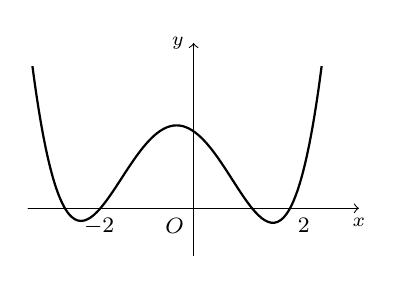
\begin{tikzpicture}[=>stealth,line join=round,line cap=round, font=\footnotesize,scale=.6]
\def\a{0.12} % Hệ số a phải khác 0
\def\b{0.17}
\def\c{-0.9}
\def\d{-0.69}
\def\e{1.63}
%\draw[color=gray,dash pattern=on 1pt off 1pt,xstep=1.0cm,ystep=1.0cm] (-5.2,-5.2) grid (5.2,5.2);
\draw[->] (-3.5,0) -- (3.5,0)node[below]{\scriptsize $x$};
\draw[->] (0,-1) -- (0,3.5) node[left] {\scriptsize $y$};
\draw (0,0)node[below left]{$O$}(-2,0)node[below]{$-2$}(2,0)node[below right]{$2$};
\clip (-3.5,-1)rectangle(3,3);
\draw[thick,samples=150,smooth,domain=-5:5] plot(\x,{\a*(\x)^4+(\b)*(\x)^3+(\c)*(\x)^2+(\d)*\x+(\e)});
\end{tikzpicture}
	
}
	\loigiai{
Ta có $g'(x)=(3x^2-3)\cdot f'(x^3-3x)=0\Leftrightarrow\hoac{&3x^2-3=0\\&f'(x^3-3x)=0}\Leftrightarrow\hoac{&x=\pm 1\\&x^3-3x=a& a\in (-3;-2)\\&x^3-3x=b& b\in (-2;0)\\&x^3-3x=c& c\in (1;2).}$\\
Bảng biến thiên của hàm số $y=x^3-3x$
\begin{center}
	\begin{tikzpicture}[>=stealth]
	\tkzTabInit[nocadre=false,lgt=1,espcl=2,deltacl=0.5]{$x$/.7 ,$y'$/.7,$y$/2}
	{$-\infty$ , $-1$ , $1$ , $+\infty$}
	\tkzTabLine{ , + , $0$ , - , $0$ , + , }
	\tkzTabVar{-/$-\infty$ , +/$2$ , -/$-2$ , +/$+\infty$}
	\begin{scope}[on background layer]\path[white]node{MDD-108};\end{scope}
\end{tikzpicture}
\end{center}
\begin{itemize}
	\item Phương trình $x^3-3x=a$ với $a\in (-3;-2)$ có $1$ nghiệm.
	\item Phương trình $x^3-3x=b$ với $b\in (-2;0)$ có $3$ nghiệm.
	\item Phương trình $x^3-3x=c$ với $c\in (1;2)$ có $3$ nghiệm.
\end{itemize}
Vậy hàm số $g(x)$ có $9$ điểm cực trị.
}
\end{ex}

\begin{ex}%[KSCL THPT Đội Cấn - Vĩnh Phúc, 2021]%[Nguyễn Cường, 12EX3]%[2D1K1-1]
Cho hàm số $y=f(x)$ có đạo hàm $f'(x)=(3-x)(10-3x)^2(x-2)^2$ với mọi $x \in \mathbb{R}$. Hàm số $g(x)=f(3-x)+\dfrac{1}{6}\left(x^2-1\right)^3$ đồng biến trên khoảng nào trong các khoảng sau?
	\choice
	{$(1;+\infty)$}
	{$(0);1$}
	{$(-\infty;0)$}
	{\True $\left(-\infty;-\dfrac{1}{2}\right)$}
	\loigiai{
		\allowdisplaybreaks
		\begin{eqnarray*}
		g'(x)&=&-f'(3-x)+\dfrac{1}{2}\cdot 2x\cdot (x^2-1)^2\\
		&=&-x(3x+1)^2(x-1)^2+x(x-1)^2(x+1)^2\\
		&=& x(x-1)^2\left((x+1)^2-(3x+1)^2\right)\\
		&=&-2x^2(x-1)^2(4x+2)
		\end{eqnarray*}
Xét $g'(x)>0\Leftrightarrow 4x+2<0 \Leftrightarrow x<-\dfrac{1}{2}$.\\
Vậy hàm số đồng biến trên khoảng $\left(-\infty;-\dfrac{1}{2}\right)$.
}
\end{ex}

\begin{ex}%[KSCL THPT Đội Cấn - Vĩnh Phúc, 2021]%[Nguyễn Cường, 12EX3]%[2D1K2-5]
\immini{Đồ thị hình bên là đồ thị của hàm số nào?
	\choice
	{$y=\dfrac{x+2}{x+1}$}
	{\True $y=\dfrac{2x+1}{x+1}$}
	{$y=\dfrac{2x-1}{x+1}$}
	{$y=\dfrac{x+3}{1-x}$}
}
{
% Đồ thị hàm y=(ax+b)/(cx+d), ad-bc khác 0. Nếu hệ số lớn cần điều chỉnh hệ trục, vùng lưới, domain và lệnh \clip
\begin{tikzpicture}[=>stealth,line join=round,line cap=round, font=\footnotesize,scale=.6]
\def\a{2}
\def\b{1}
\def\c{1}
\def\d{1}
%\draw[color=gray,dash pattern=on 1pt off 1pt,xstep=1.0cm,ystep=1.0cm] (-5.2,-5.2) grid (5.2,5.2);
\draw[->] (-4.3,0) -- (2.3,0) node[below] {\scriptsize $x$};
\draw[->] (0,-2.3) -- (0,5.3) node[left] {\scriptsize $y$};
\draw (0,0)node[below right]{$O$} (-1,0)node[below left]{$-1$} (0,2)node[above left]{$2$};
\draw[dashed,blue] (-1,-2.3)--(-1,5.3) (-4.3,2)--(2.3,2); % Vẽ TCĐ và TCN
\clip (-4,-2)rectangle(2,5);
\pgfmathsetmacro{\can}{-(\d)/(\c)}
\draw[thick,samples=150,smooth,domain=-5:{\can-.1}] plot(\x,{(\a*\x+(\b))/(\c*\x+(\d))}); % Vẽ nhánh bên trái TCĐ
\draw[thick,samples=150,smooth,domain={\can+.1}:5] plot(\x,{(\a*\x+(\b))/(\c*\x+(\d))}); % Vẽ nhánh bên phải TCĐ
\end{tikzpicture}
}
	\loigiai{
Đồ thị hàm số $y=\dfrac{2x+1}{x+1}$ có đường tiệm cận ngang và đường tiệm cận đứng lần lượt là $y=2$; $x=-1$.\\
Đồ thị hàm số $y=\dfrac{2x+1}{x+1}$ đi qua điểm $(0;1)$.\\
Hàm số $y=\dfrac{2x+1}{x+1}$ đồng biến trên từng khoảng xác định.
	}
\end{ex}

\begin{ex}%[KSCL THPT Đội Cấn - Vĩnh Phúc, 2021]%[Nguyễn Cường, 12EX3]%[2D1K1-3]
Có tất cả bao nhiêu số nguyên dương $m$ để hàm số $y=\dfrac{\cos x+1}{10\cos x+m}$ đồng biến trên khoảng $\left(0;\dfrac{\pi}{2}\right)$?
	\choice
	{\True $9$}
	{$8$}
	{$10$}
	{$11$}
	\loigiai{
Đặt $t=\cos x$, với $x \in \left(0;\dfrac{\pi}{2}\right)$ thì $t\in (0;1)$.\\
$t'=-\sin x<0$ với mọi $x \in \left(0;\dfrac{\pi}{2}\right)$.\\
Khi đó bài toán trở thành $y=\dfrac{t+1}{10t+m}$ nghịch biến trên khoảng $(0;1)$.\\
Điều kiện $t\ne -\dfrac{m}{10}$.\\
Đạo hàm $y'=\dfrac{m-10}{(10t+m)^2}$.\\
Hàm số nghịch biến trên khoảng $(0;1)$ $\Leftrightarrow\heva{&m-10<0\\&\hoac{&-\dfrac{m}{10}\ge 1\\&-\dfrac{m}{10}\le 0}}\Leftrightarrow \heva{&m<10\\&\hoac{&m\le -10\\&m\ge 0}}\Leftrightarrow \hoac{&m\le -10\\&0\le m<10.}$\\
Vậy $m\in \{1;2;3;\ldots;9\}$ nên có $9$ giá trị nguyên dương của $m$.
	}
\end{ex}

\begin{ex}%[KSCL THPT Đội Cấn - Vĩnh Phúc, 2021]%[Nguyễn Cường, 12EX3]%[2H1K3-2]
	Cho hình chóp $S.ABC$ có $SA$ vuông góc với mặt phẳng $(ABC)$, $SA=1$ và đáy $ABC$ là tam giác đều với độ dài cạnh bằng $2$. Tính góc giữa mặt phẳng $(SBC)$ và mặt phẳng $(ABC)$.
	\choice
	{$90^\circ$}
	{$60^\circ$}
	{$45^\circ$}
	{\True $30^\circ$}
	\loigiai{
\immini
{
Gọi $M$ là trung điểm $BC$.\\
Ta có $\heva{&(SBC)\cap (ABC)=BC\\&BC\perp AM\\&BC\perp SM}$ suy ra góc giữa mặt phẳng $(SBC)$ và mặt phẳng $(ABC)$ là $\widehat{SMA}$.\\
Xét $\triangle SAM$ vuông tại $A$ có	
$\tan\widehat{SMA}=\dfrac{SA}{AM}=\dfrac{1}{\sqrt{3}}$ suy ra $\widehat{SMA}=30^\circ$. 
} 
{
	\begin{tikzpicture}[=>stealth,line join=round,line cap=round, font=\footnotesize, scale=.7]
	\def\a{4}
	\def\goc{210}
	\def\b{3}
	\def\h{4}
	\path
	(0,0)coordinate (A)++(0:\a)coordinate (B)++(\goc:\b)coordinate (C)
	(A)++(90:\h)coordinate (S)
	($(B)!.5!(C)$)coordinate (M)
	;
	\draw (S)--(A)--(C)--(B)--cycle
	(M)--(S)--(C)
	;
	\draw[dashed] (M)--(A)--(B);
	\foreach \x/\g in{A/180,B/45,C/-60,S/90,M/-45}
	\fill[black](\x)circle(1.5pt) ($(\x)+(\g:3mm)$)node{$\x$}
	;
	\begin{scope}[on background layer]\path[white]node{MDD-108};\end{scope}
\end{tikzpicture}
}		
}
\end{ex}

\begin{ex}%[KSCL THPT Đội Cấn - Vĩnh Phúc, 2021]%[Nguyễn Cường, 12EX3]%[2H1K3-2]
Tiếp tuyến của đồ thị hàm số $y=x^3+2x^2-3$ tại điểm $A(1;0)$ có hệ số góc bằng
	\choice
	{\True $7$}
	{$-7$}
	{$-1$}
	{$1$}
	\loigiai{
Đạo hàm $y'=3x^2+4x$, hệ số góc của tiếp tuyến tại $A(1;0)$ là $k=y'(1)=7$.
	}
\end{ex}

\begin{ex}%[Khảo sát Toán 12 - THPT Đội Cấn -Vĩnh Phúc - 21]%[Phan Văn Thành]%[2H1K3-6]
	Một công ty cần xây một kho chứa hàng dạng hình hộp chữ nhật (bằng vật liệu gạch và xi măng) có thể tích $2000$ m$^3$, đáy là hình chữ nhật có chiều dài bằng hai lần chiều rộng. Người ta cần tính toán sao cho chi phí xây dựng là thấp nhất, biết giá xây dựng là $750000$ đ/m$^2$. Khi đó chi phí thấp nhất gần với số nào dưới đây?
	\choice
	{$ 742.935.831 $}
	{$ 742.963.631 $}
	{\True $ 742.933.631 $}
	{$ 742.833.631 $}
	\loigiai{
	Gọi chiều rộng của đáy hình chữ nhật là $x$, $(x>0)$. Khi đó chiều dài của đáy là $2x$.\\
	Gọi chiều cao của kho chứa dạng hình hộp chữ nhật là $h$, ($h>0$).\\
	Khi đó $V = h\cdot x\cdot 2x \Leftrightarrow 2000 = 2x^2h \Rightarrow h = \dfrac{1000}{x^2}$.\\
	Để chi phí xây dựng là thấp nhất thì diện tích toàn phần của kho chứa là nhỏ nhất.\\
\immini{	Ta có \begin{eqnarray*}
	 S_{\text{Tp}} 	&= & S_{\text{xq}} + 2S_{\text{đáy}}\\
		&= & 6xh+4x^2 = \dfrac{6000}{x} + 4x^2\\
		&= & \dfrac{3000}{x}+ \dfrac{3000}{x} + 4x^2\\
		&\geq & 3\sqrt[3]{\dfrac{3000}{x} \cdot \dfrac{3000}{x} \cdot 4x^2} = 300\sqrt[3]{36}.
	\end{eqnarray*}}{\begin{tikzpicture}[scale=.7, line join = round, line cap = round]
\tikzset{label style/.style={font=\footnotesize}}
\tkzDefPoints{0/0/A,6/0/B,-2/-2/D}
\coordinate (C) at ($(B)+(D)-(A)$);
\coordinate (A') at ($(A) - (0,3.5)$);
\tkzDefPointsBy[translation = from A to A'](B,C,D){B'}{C'}{D'}
\tkzDrawPolygon(A,B,B',C',D',D)
\tkzDrawSegments(C,B C,D C,C')
\tkzDrawSegments[dashed](A',A A',B' A',D')
\tkzDrawPoints[fill=black](A,B,D,C,A',B',C',D')
\tkzLabelSegment[left](D,D'){$h$}
\tkzLabelSegment[left](D,A){$x$}
\tkzLabelSegment[above](D,C){$2x$}
\end{tikzpicture}}
Dấu đẳng thức xảy ra khi và chỉ khi $\dfrac{3000}{x} = 4x^2 \Leftrightarrow x = \sqrt[3]{750}$.\\
Vậy chi phí xây dựng thấp nhất là $300\sqrt[3]{36}\cdot 750000 = 742933631$ (đồng).
	}
\end{ex}

\begin{ex}%[KSCL THPT Đội Cấn - Vĩnh Phúc, 2021]%[Nguyễn Cường, 12EX3]%[2D1K4-1]
 Cho hàm số $y=f(x)$ có bảng xét dấu đạo hàm như sau
 \begin{center}
 	% Cần khai báo \usepackage{tkz-tab}
 	\begin{tikzpicture}
 	\tkzTabInit[nocadre=false,lgt=2,espcl=2,deltacl=0.5]{$x$/1 ,$f'(x)$/1}
 	{$-\infty$ , $1$ , $2$ , $3$ , $4$ , $+\infty$}
 	\tkzTabLine{  , - , z , + , 0 ,  + ,z,  - , z , + }
  	\begin{scope}[on background layer]\path[white]node{MDD-108};\end{scope}
\end{tikzpicture}
 	 \end{center}
Biết rằng $f(2)+f(6)=2f(3)$. Tập nghiệm của phương trình $f(x^2+1)=f(3)$ có số phần tử bằng
	\choice
	{$5$}
	{$3$}
	{$2$}
	{\True  $4$}
	\loigiai{
		
Ta có $g'(x)=2x\cdot f'(x^2+1)=0\hoac{&x=0\\&x^2+1=1\\&x^2+1=2\\&x^2+1=3\\&x^2+1=4}\Leftrightarrow\hoac{&x=0\\&x=\pm 1\\&x=\pm\sqrt{2}\\&x=\pm\sqrt{3}.}$\\
Bảng biến thiên 
\begin{center}
	\begin{tikzpicture}[every node/.style={circle,fill=white,inner sep=0pt},arrow/.style={>=stealth,->,shorten <= 0.3cm,shorten >= 0.3cm},font=\footnotesize,xscale=1,yscale=.6]
	\def\mnumline{6} %Số dòng
	\def\mnumcol{17} %Số cột
	\foreach \j in {0,...,\mnumline}
	\foreach \i in {0,...,\mnumcol}{
		\coordinate (\j\i) at (\i,-\j);
%		\draw[gray!30] ([xshift=-0.5cm,yshift=0.5cm]\j\i)--([xshift=0.5cm,yshift=0.5cm]\j\i)--([xshift=0.5cm,yshift=-0.5cm]\j\i)--([xshift=-0.5cm,yshift=-0.5cm]\j\i)--cycle (\j\i)node[]{\j\i}; %Ẩn lệnh này sau khi hoàn thành BBT
	}
	\pgfmathsetmacro\yline{\mnumline/2-1}
	\path node at (00){$x$} node at (10){$y'$} node at ([yshift=\yline cm]\mnumline0){$y$};
	\foreach \x/\mnamex in {01/$-\infty$,03/$-\sqrt{3}$,05/$-\sqrt{2}$,07/$-1$,09/$0$,011/$1$,013/$\sqrt{2}$,015/$\sqrt{3}$,0\mnumcol/$+\infty$} \path node at (\x) {\mnamex};
	\foreach \dy/\mnamedy in {12/$-$,13/$0$,14/$+$,15/$0$,16/$-$,17/$0$,18/$-$,19/$0$,110/$+$,111/$0$,112/$+$,113/$0$,114/$-$,115/$0$,116/$+$} \path node at (\dy) {\mnamedy};
	\path 
	node at ($(21)$){$+\infty$} 
	node at ($(63)$){$f(4)$} 
	node at ($([yshift=-.2cm]25)$){$f(3)$}
	node at ($([yshift=.5cm]47)$){$f(2)$} 
	node at ($(69)$){$f(1)$} 
	node at ($([yshift=.5cm]411)$){$f(2)$}
	node at ($([yshift=-.2cm]213)$){$f(3)$} 
	node at ($(615)$){$f(4)$} 
	node at ($(217)$){$+\infty$}	
	;
%	\path[pattern=north east lines] ([yshift=0.5cm]$(25)$)rectangle([xshift=0.5cm,yshift=-0.5cm]$(67)$); %Vẽ vùng bỏ đi
%	\draw[double,double distance=2pt] ([yshift=0.5cm]$(15)$)--([yshift=-0.5cm]$(65)$); %Vẽ các đường nét đôi (không xác định)
	\draw[cyan,arrow] ($(21)$)--($(63)$);
	\draw[cyan,arrow] ($(63)$)--($(25)$);
	\draw[cyan,arrow] ($(25)$)--([xshift=-.2cm]$(69)$);
	\draw[cyan,arrow] ($(69)$)--($(213)$);
	\draw[cyan,arrow] ($(213)$)--([xshift=-.2cm]$(615)$);
	\draw[cyan,arrow] ($(615)$)--($(217)$);
%	\draw[cyan,arrow] ($(25)$)--([xshift=-.2cm]$(69)$);
	\draw[thick] (-.5,.5)rectangle([xshift=0.5cm,yshift=-0.5cm]\mnumline\mnumcol) ([xshift=-0.5cm,yshift=-0.5cm]00)--([xshift=0.5cm,yshift=-0.5cm]0\mnumcol) ([xshift=-0.5cm,yshift=-0.5cm]10)--([xshift=0.5cm,yshift=-0.5cm]1\mnumcol) ([xshift=0.5cm,yshift=0.5cm]00)--([xshift=0.5cm,yshift=-0.5cm]\mnumline0); %Lệnh tự động kẻ bảng
	\begin{scope}[on background layer]\path[white]node{MDD-108};\end{scope}
\end{tikzpicture}
\end{center}
}
\end{ex}
\Closesolutionfile{ans}
\begin{indapan}{10}
	{ans/ans-2-GHK1-21-KSCLDoiCanVinhPhuc-21}
\end{indapan}
